% Nafs-Aql Development Roadmap. Build: ../../tools/tectonic nafs_aql_roadmap.tex
\documentclass[11pt,a4paper]{article}
\usepackage[margin=2.2cm]{geometry}
\usepackage[utf8]{inputenc}\usepackage[T1]{fontenc}
\usepackage{amsmath,amssymb}
\usepackage{booktabs,array,longtable}
\usepackage{graphicx,xcolor}
\usepackage{tikz,pgfplots}\pgfplotsset{compat=1.18}
\usetikzlibrary{arrows.meta,positioning,shapes.geometric,fit,calc,backgrounds}
\usepackage{enumitem}\setlist{nosep,leftmargin=*}
\usepackage{microtype}\usepackage{url}\usepackage[hidelinks,pdfauthor={Dirac R\&D Team}]{hyperref}\usepackage{fancyhdr}
% Shared palette, TikZ styles and macros for all Nafs-Aql documents
\definecolor{navy}{HTML}{1F3A5F}
\definecolor{teal}{HTML}{1B8A8F}
\definecolor{amber}{HTML}{C97D10}
\definecolor{crimson}{HTML}{B3263E}
\definecolor{violet}{HTML}{6A4C9C}
\definecolor{leaf}{HTML}{3A8F4B}
\definecolor{slate}{HTML}{5B6770}
\definecolor{sand}{HTML}{F4EFE6}
\tikzset{
  blk/.style={rounded corners=2.5pt,draw=#1!85!black,fill=#1!12,thick,align=center,
              font=\scriptsize,inner sep=3pt,minimum height=0.72cm},
  blk/.default=navy,
  sblk/.style={rounded corners=2.5pt,draw=#1!85!black,fill=#1!12,thick,align=center,
              font=\tiny,inner sep=2pt,minimum height=0.55cm},
  sblk/.default=navy,
  dm/.style={diamond,aspect=2.2,draw=amber!85!black,fill=amber!15,thick,font=\tiny,
             align=center,inner sep=0.5pt},
  st/.style={circle,draw=#1!85!black,fill=#1!15,thick,font=\scriptsize,minimum size=0.78cm,inner sep=0pt},
  st/.default=navy,
  arr/.style={-{Stealth[length=4pt,width=3pt]},thick,draw=slate},
  dsh/.style={-{Stealth[length=4pt,width=3pt]},thick,dashed,draw=slate!80},
  lab/.style={font=\tiny,fill=white,inner sep=1pt,text=black!80},
  grp/.style={rounded corners=4pt,draw=#1!60,dashed,thick,inner sep=5pt,fill=#1!4},
  grp/.default=slate,
  grplab/.style={font=\tiny\bfseries,text=#1!80!black,anchor=north west,inner sep=2pt},
  grplab/.default=slate
}
\pgfplotsset{every axis/.append style={font=\scriptsize,grid=major,grid style={black!10},
  legend style={font=\tiny,draw=none,fill=white,fill opacity=.85,text opacity=1},
  tick label style={font=\tiny},label style={font=\scriptsize}}}
% ---- shared names (single source of truth) ----
\newcommand{\Sys}{Nafs-Aql}
\newcommand{\Sone}{System~1}
\newcommand{\Stwo}{System~2}
\newcommand{\Gate}{Aql Gate}
\newcommand{\Hub}{Verifier Hub}
\newcommand{\Ledger}{Muhasaba Ledger}
\newcommand{\Distil}{Tazkiya Distillation}
\newcommand{\Mem}{Context Manager}
\newcommand{\Gw}{Rust Gateway}
\newcommand{\Harness}{Eval Harness}

\newcommand{\ReqsPhaseA}{FR-050, NFR-012, NFR-023, MR-001, MR-003, MR-005, OR-001, ER-001, ER-010, ER-011}
\newcommand{\ReqsPhaseB}{FR-001, FR-002, FR-003, FR-005, FR-006, FR-012, FR-013, FR-023, FR-024, FR-026, FR-030, FR-031, FR-035, FR-060, NFR-001, NFR-002, NFR-003, NFR-004, NFR-005, NFR-006, NFR-011, NFR-021, NFR-022, IF-001, IF-002, IF-003, IF-004, IF-005, IF-006, IF-007, IF-008, IF-010, MR-002, SR-002, OR-006, ER-006}
\newcommand{\ReqsPhaseC}{FR-004, FR-010, FR-011, FR-014, FR-015, FR-020, FR-021, FR-022, FR-025, FR-032, FR-034, FR-040, FR-041, NFR-010, NFR-020, MR-004, SR-001, SR-003, ER-002, ER-003, ER-004, ER-005}
\newcommand{\ReqsPhaseD}{FR-033, FR-070, TR-001, TR-002, TR-003, TR-004, TR-005, TR-006, TR-007, TR-008, SR-004, OR-005, ER-008}
\newcommand{\ReqsPhaseE}{FR-042, FR-051, FR-052, FR-053, NFR-007, IF-009, ER-007}
\newcommand{\ReqsPhaseF}{FR-061, SR-006, OR-002, OR-003, OR-004}
\newcommand{\ReqsPhaseG}{SR-005}
\newcommand{\ReqsPhaseH}{NFR-030, NFR-031, FR-080, FR-081, ER-020, FR-082}
\newcommand{\TasksPhaseA}{
\begin{tabular}{@{}p{1.1cm}p{2.3cm}p{6.0cm}p{0.9cm}p{1.9cm}p{1.7cm}@{}}
\toprule ID & Epic & Task & PW & Depends & MoSCoW\\\midrule
P0-T01 & E0.1 Environment & Build llama.cpp and vLLM-CPU container; publish serving recipes for Profile A & 1.0 & -- & Must\\
P0-T02 & E0.1 Environment & Pin model revisions, GGUF hashes, chat-template hashes; write model manifest & 0.5 & P0-T01 & Must\\
P0-T03 & E0.2 Measurement & Implement minimal Eval Harness (dataset loaders, exact verifiers for GSM8K/HumanEval/schema, metrics) & 2.0 & P0-T01 & Must\\
P0-T04 & E0.2 Measurement & Run fast-only and slow-only baselines on $\ge$ 4600 tasks; fit q, (r,phi), e1(s), e2(s), cost ratio, discordance & 1.5 & P0-T03 & Must\\
P0-T05 & E0.2 Measurement & Measure accuracy vs thinking budget per domain (H4) and acceptance-rate distribution & 1.0 & P0-T04 & Must\\
P0-T06 & E0.3 Hybrid gate & llama-bench Qwen3.5-2B/4B vs Qwen3-1.7B/4B on target CPU (H7); decide Profile C & 0.5 & P0-T01 & Must\\
P0-T07 & E0.4 Workspace & Create Cargo workspace, CI (fmt, clippy, test on Linux and macOS), config schema & 1.0 & -- & Must\\
\bottomrule\end{tabular}}
\newcommand{\TasksPhaseB}{
\begin{tabular}{@{}p{1.1cm}p{2.3cm}p{6.0cm}p{0.9cm}p{1.9cm}p{1.7cm}@{}}
\toprule ID & Epic & Task & PW & Depends & MoSCoW\\\midrule
P1-T01 & E1.1 Gateway & axum gateway: /v1/chat, /v1/chat/stream (SSE), auth, rate limit, metrics, OpenAPI at /openapi.json & 2.0 & P0-T07 & Must\\
P1-T02 & E1.2 Backends & Backend trait + llama-server and vLLM implementations: logprobs, parallel samples, thinking toggle, retry, semaphore & 2.0 & P0-T07 & Must\\
P1-T03 & E1.3 Orchestrator & Trace-state automaton with fixed-rule gate, budget forcing, caps, decision record, assurance levels & 2.5 & P1-T02 & Must\\
P1-T04 & E1.4 Verifiers & Verifier Hub v1: code sandbox (subprocess limits), JSON Schema verifier & 2.0 & P0-T07 & Must\\
P1-T05 & E1.5 Memory & SQLite conversation store, JSONL traces, context cap and prompt-cache prefix preservation & 1.5 & P0-T07 & Must\\
P1-T06 & E1.6 Web UI & Chat room UI (askama + htmx + WebSocket), reasoning mode and assurance badges, controller event stream & 2.0 & P1-T01 & Must\\
P1-T07 & E1.7 MVP acceptance & Profile selection, MVP acceptance tests, latency targets measured on reference machine & 1.0 & P1-T03, P1-T04, P1-T05, P1-T06 & Must\\
\bottomrule\end{tabular}}
\newcommand{\TasksPhaseC}{
\begin{tabular}{@{}p{1.1cm}p{2.3cm}p{6.0cm}p{0.9cm}p{1.9cm}p{1.7cm}@{}}
\toprule ID & Epic & Task & PW & Depends & MoSCoW\\\midrule
P2-T01 & E2.1 Calibrated gate & Feature extraction, logistic/isotonic estimator, cost-ratio rule, budget mode, recalibration job & 2.5 & P0-T04, P1-T03 & Must\\
P2-T02 & E2.2 Verified loop & Sequential verified sampling, evidence-fed retries, caps from Beta fit, R$\le$1 on non-verifiable & 2.0 & P1-T03, P0-T05 & Must\\
P2-T03 & E2.3 Verifier quality & Math verifier (numeric + SymPy sidecar), mutation-testing harness, (r,phi) publication, judge hard gate & 2.0 & P1-T04 & Must\\
P2-T04 & E2.4 Audit and ledger & 5 percent audit stream, capability table with unmeasured labels, adapter-hash keying & 1.5 & P2-T01 & Must\\
P2-T05 & E2.5 Resilience & Backend reconnect, degraded mode, prompt-injection delimiting & 1.0 & P1-T02 & Must\\
P2-T06 & E2.6 Gate G2 evaluation & Coupling test ($\ge$ 200 trials), calibration test ($\ge$ 2900), 3-point non-inferiority ($\ge$ 700 pairs) & 1.5 & P2-T01, P2-T02, P2-T03 & Must\\
\bottomrule\end{tabular}}
\newcommand{\TasksPhaseD}{
\begin{tabular}{@{}p{1.1cm}p{2.3cm}p{6.0cm}p{0.9cm}p{1.9cm}p{1.7cm}@{}}
\toprule ID & Epic & Task & PW & Depends & MoSCoW\\\midrule
P3-T01 & E3.1 Data pipeline & Dataset builder from verified traces; schema; dedupe; domain cap; abstain and replay mixing; privacy redaction & 1.5 & P2-T04 & Must\\
P3-T02 & E3.2 Synthetic data & System 2 synthetic generation on benchmark-like prompts with held-out verifier & 1.0 & P3-T01 & Should\\
P3-T03 & E3.3 Unsloth training & Unsloth LoRA scripts, GPU runbook (T4), checkpoint and adapter hashing, GGUF export & 1.5 & P3-T01 & Must\\
P3-T04 & E3.4 Promotion & Promotion gate with confidence bounds, regression suite, human sign-off, one-command rollback & 1.5 & P3-T03 & Must\\
\bottomrule\end{tabular}}
\newcommand{\TasksPhaseE}{
\begin{tabular}{@{}p{1.1cm}p{2.3cm}p{6.0cm}p{0.9cm}p{1.9cm}p{1.7cm}@{}}
\toprule ID & Epic & Task & PW & Depends & MoSCoW\\\midrule
P4-T01 & E4.1 Statistics & Paired tests, CIs, non-inferiority, Bonferroni in harness; report export & 1.5 & P2-T06 & Must\\
P4-T02 & E4.2 Performance console & goose load generator, bench runs API, latency quantiles, concurrency protocol & 2.0 & P1-T01 & Must\\
P4-T03 & E4.3 Dashboard & Evaluation dashboard: runs, calibration plots, routing accuracy, gate status & 2.0 & P4-T01 & Should\\
P4-T04 & E4.4 Drift & CUSUM drift monitor with negative control on ledger & 1.0 & P2-T04 & Should\\
\bottomrule\end{tabular}}
\newcommand{\TasksPhaseF}{
\begin{tabular}{@{}p{1.1cm}p{2.3cm}p{6.0cm}p{0.9cm}p{1.9cm}p{1.7cm}@{}}
\toprule ID & Epic & Task & PW & Depends & MoSCoW\\\midrule
P5-T01 & E5.1 Hardening & Security review, TLS and secrets, sandbox escape tests, packaging with manifest & 2.0 & P4-T02 & Must\\
P5-T02 & E5.2 Deployment & docker-compose (vLLM-CPU) and service files (llama-server); monitoring and alerts & 1.5 & P5-T01 & Must\\
P5-T03 & E5.3 GPU scale-out & vLLM CUDA profile with both models resident, higher N and budget, speculative decoding & 1.5 & P5-T02 & Could\\
P5-T04 & E5.4 Upgrade decision & Profile C (Qwen3.5) evaluation on full suite; optional retrieval memory & 1.5 & P0-T06, P4-T01 & Could\\
\bottomrule\end{tabular}}
\newcommand{\TasksPhaseG}{
\begin{tabular}{@{}p{1.1cm}p{2.3cm}p{6.0cm}p{0.9cm}p{1.9cm}p{1.7cm}@{}}
\toprule ID & Epic & Task & PW & Depends & MoSCoW\\\midrule
P6-T01 & E6.1 Release gate & 1-point non-inferiority on $\ge$ 6200 pairs; full regression; scholar review of analogy copy & 2.0 & P5-T01 & Must\\
P6-T02 & E6.2 Documentation & Operator and user documentation; API reference; runbooks & 1.0 & P6-T01 & Must\\
P6-T03 & E6.3 Publication & Research write-up with measured results; artefact release & 1.5 & P6-T01 & Should\\
\bottomrule\end{tabular}}
\newcommand{\TasksPhaseH}{
\begin{tabular}{@{}p{1.1cm}p{2.3cm}p{6.0cm}p{0.9cm}p{1.9cm}p{1.7cm}@{}}
\toprule ID & Epic & Task & PW & Depends & MoSCoW\\\midrule
P7-T01 & E7.1 Observability & Per-stage latency with server prefill/decode/cache split; /v1/perf/stages; inspector waterfall and Performance breakdown & 1.0 & P4-T02 & Must\\
P7-T02 & E7.2 Engine & Interleaved A/B harness and study of flash attention, BLAS prefill, KV-cache type and threads; verifier warm-up & 1.0 & P7-T01 & Must\\
P7-T03 & E7.3 Cascade & Early escalation in the streaming draft (fixed rule) with decision-agreement study & 1.0 & P7-T01 & Should\\
P7-T04 & E7.2 Engine & EAGLE-3 heads for Qwen3-1.7B and Qwen3-4B (convert, serve, measure acceptance and speed-up) & 1.0 & P7-T02 & Could\\
P7-T05 & E7.2 Engine & Weight-format study: Q4\_0 / IQ4\_NL with AVX2 repack kernels against Q4\_K\_M (speed and accuracy on regression\_500) & 1.0 & P7-T02 & Could\\
P7-T06 & E7.4 Lab & Efficiency frontier in Lab insights: early escalation, saved tokens, routing agreement per domain & 1.0 & P7-T03 & Should\\
P7-T07 & E7.5 Release & End-to-end sweep, UI screenshots, technical report and slides refresh, forward roadmap & 1.0 & P7-T06 & Must\\
P7-T08 & E7.3 Cascade & Adaptive reasoning exit: probe-and-verify on the raw continuation path, with a token-saving study & 1.0 & P7-T03 & Should\\
P7-T09 & E7.3 Cascade & Judge on System 1: measure the small judge's (r, phi) with the rates harness and adopt it if the rates hold & 0.5 & P7-T01 & Could\\
P7-T10 & E7.6 Backends & vLLM CPU backend in Docker (carstenz/vllm-smoke image, BF16, one model in two modes) with an end-to-end check against the gateway & 1.0 & P5-T02 & Should\\
\bottomrule\end{tabular}}
\newcommand{\TasksPhaseI}{
\begin{tabular}{@{}p{1.1cm}p{2.3cm}p{6.0cm}p{0.9cm}p{1.9cm}p{1.7cm}@{}}
\toprule ID & Epic & Task & PW & Depends & MoSCoW\\\midrule
P8-T01 & E8.1 Evidence & Confidence-signal study: which token-level signal of a System 1 draft predicts a wrong draft (ROC against exact labels) & 0.5 & P7-T03 & Should\\
P8-T02 & E8.1 Evidence & Lowest-window confidence as a gate feature and an exact early-escalation rule (running minimum) & 0.5 & P8-T01 & Should\\
P8-T03 & E8.2 Deliberation & Posterior stopping rule with a collapsing bound for the adaptive exit on non-verifiable tasks & 0.5 & P7-T08 & Could\\
P8-T05 & E8.1 Evidence & Agreement samples on unverified mathematics drafts (adopted from the study's agreement arm) & 0.25 & P8-T01 & Should\\
P8-T04 & E8.3 Research & Quantum-consciousness and neuroscience review with first-principles verdicts and the sequential-evidence propositions & 0.5 & -- & Should\\
\bottomrule\end{tabular}}
\newcommand{\TasksPhaseJ}{
\begin{tabular}{@{}p{1.1cm}p{2.3cm}p{6.0cm}p{0.9cm}p{1.9cm}p{1.7cm}@{}}
\toprule ID & Epic & Task & PW & Depends & MoSCoW\\\midrule
P9-T01 & E9.1 Rooms & Room store and API: unique normalised names, rename, delete with a full ledger purge, activity and presence in the list & 1.0 & -- & Must\\
P9-T02 & E9.1 Rooms & Room hub: welcome snapshot with cursor and pending turns, unique display names, queue and typing frames, heartbeat, race-safe deletion & 1.0 & P9-T01 & Must\\
P9-T03 & E9.2 Rooms UI & Rooms page rebuilt: list with search and unread, deep links, inline rename, confirmed delete, export, reconnecting transcript, drafts, mobile drawer & 1.5 & P9-T02 & Should\\
P9-T04 & E9.3 Verification & Live rooms test with simulated members; sweep checks; screenshots; API contract and documents & 0.5 & P9-T03 & Should\\
\bottomrule\end{tabular}}
\newcommand{\PWTotals}{P0: 7.5; P1: 13.0; P2: 10.5; P3: 5.5; P4: 6.5; P5: 6.5; P6: 4.5; P7: 9.5; P8: 2.2; P9: 4.0}
\newcommand{\PWGrand}{69.8}
\newcommand{\NTasks}{54}
\newcommand{\NReqs}{109}

\pagestyle{fancy}\fancyhf{}\lhead{\small Nafs-Aql Development Roadmap v2.0}\rhead{\small Dirac R\&D Team}\cfoot{\small\thepage}
\title{\textbf{Nafs-Aql Development Roadmap}\\[4pt]\large Version 2.1 (20 October 2026): Phases 0--6 implemented, Phases 7--8 added, road ahead}
\author{Dirac R\&D Team}\date{}
\begin{document}\maketitle
\begin{abstract}\noindent
This roadmap takes \Sys\ from the current draft to a production-ready release in seven phases. Each phase has objectives, scope, deliverables, work packages with task identifiers, dependencies, measurable entry and exit criteria, and the requirement identifiers from the Technical Specification that it satisfies. Milestones are decision gates with explicit go/no-go criteria and fallbacks. The minimum viable product is defined with acceptance tests. Effort, duration and compute figures are \emph{estimates} under the stated assumptions. The backlog is exported as \texttt{backlog.csv} and \texttt{roadmap.md}; the task and requirement tables are generated from the same source files as the specification. Version~2.0 records where the implementation stands, adds Phase~7 (CPU inference performance) and sets out the road ahead in Section~\ref{sec:ahead}.
\end{abstract}
\tableofcontents\clearpage

\section{Overview}
\subsection{Phases and timeline}
\begin{figure}[h]\centering\scalebox{1.6}{% Roadmap timeline (weeks); width ~8.6cm; estimates. Phase 7 was added after Phases 0-6 were implemented.
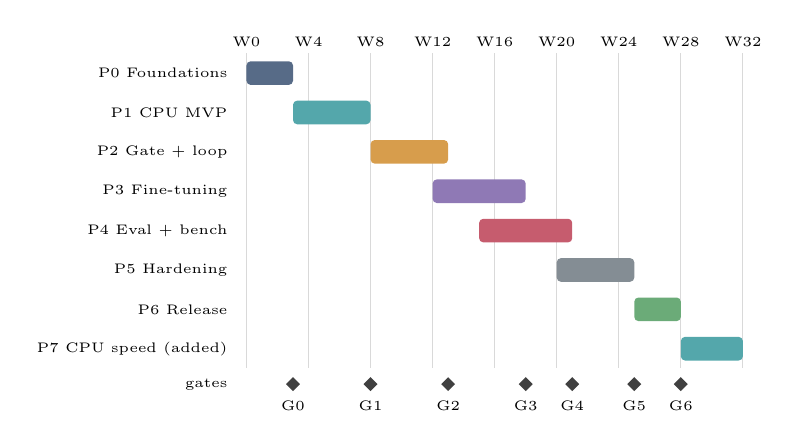
\begin{tikzpicture}[x=0.197cm,y=0.5cm]
\foreach \w in {0,4,...,32}{\draw[black!15] (\w,0.3)--(\w,-7.7);\node[font=\tiny] at (\w,0.6){W\w};}
\foreach \ii/\lbl/\st/\en/\col in {
 0/{P0 Foundations}/0/3/navy,
 1/{P1 CPU MVP}/3/8/teal,
 2/{P2 Gate + loop}/8/13/amber,
 3/{P3 Fine-tuning}/12/18/violet,
 4/{P4 Eval + bench}/15/21/crimson,
 5/{P5 Hardening}/20/25/slate,
 6/{P6 Release}/25/28/leaf,
 7/{P7 CPU speed (added)}/28/32/teal}
 {\node[anchor=east,font=\tiny] at (-0.6,-\ii-0.2){\lbl};
  \fill[\col!75,rounded corners=1.5pt](\st,-\ii-0.5) rectangle (\en,-\ii+0.1);}
\foreach \x/\n in {3/G0,8/G1,13/G2,18/G3,21/G4,25/G5,28/G6}{\node[diamond,fill=black!75,inner sep=1.3pt] (g\n) at (\x,-8.1){};\node[font=\tiny,below=1pt] at (\x,-8.2){\n};}
\node[anchor=east,font=\tiny] at (-0.6,-8.1){gates};
\end{tikzpicture}
}\caption{Timeline (weeks from project start; estimates). Diamonds are decision gates G0--G6.}\label{fig:gantt}\end{figure}
Phases overlap where their work packages are independent (for example, fine-tuning data work starts while the gate is being calibrated). Total estimated effort is \PWGrand\ person-weeks over 32 calendar weeks (28 for Phases 0--6, plus the added Phase~7) (\NTasks\ tasks; totals by phase: \PWTotals). The critical path (Figure~\ref{fig:dep}) runs through serving, the measurement baseline, the calibrated gate, the data pipeline, training, promotion, hardening and the release gate.
\subsection{Assumptions behind the estimates}
\begin{enumerate}
\item Team of three to four engineers (Section~\ref{sec:effort}) working concurrently; one GPU day per week available from Phase~3.
\item The reference CPU machine is available full time for baselines and tests; evaluation runs of 4\,600 tasks on the slow path take about two to three machine-days and are scheduled overnight.
\item Qwen3 Profile~A is the default; Profile~C is adopted only through gate G0 or G5.
\item No external dependency on model releases: pinned revisions are not changed mid-programme (any change re-runs the regression suite and, if the gate's calibration is affected, the Phase-0 baseline).
\end{enumerate}

\section{Phase 0: Foundations and Feasibility (weeks 0--3)}
\textbf{Objectives.} Serve both models on the reference machine; establish the measurement baseline that every later parameter depends on; create the workspace and CI. \textbf{Scope.} Serving recipes, model manifest, minimal harness with exact verifiers, 4\,600-task baseline run, accuracy-versus-budget curve, hybrid-model benchmark, Cargo workspace. \textbf{Deliverables.} Serving scripts (llama-server, vLLM-CPU container), \texttt{models/manifest.json}, harness v0, Phase-0 report with $q$, $(r,\varphi)$, $e_1(s)$, $e_2(s)$, cost ratio, discordance, Beta fits, budget curves, llama-bench table. \textbf{Requirements satisfied.} \ReqsPhaseA.
\par\medskip\noindent\TasksPhaseA
\par\medskip\noindent\textbf{Dependencies.} None external; P0-T03 depends on P0-T01. \textbf{Entry criteria.} Reference machine and GPU credit available; draft and report accepted. \textbf{Exit criteria (measurable).} (1)~Both Profile-A servers answer the OpenAI-compatible probe with log-probabilities and separated reasoning; (2)~baseline run of $\ge4\,600$ tasks across $\ge5$ domains completed with per-domain tables; (3)~exact verifiers for GSM8K, HumanEval and schema tasks have $\hat\varphi$ upper bound $\le0.01$ on $\ge200$ mutants; (4)~llama-bench table for Qwen3-1.7B/4B and Qwen3.5-2B/4B recorded; (5)~CI green on Linux and macOS.

\section{Phase 1: CPU-Only MVP (weeks 3--8)}
\textbf{Objectives.} The smallest build that demonstrates the idea end to end on the reference machine. \textbf{Scope.} Gateway, backends, orchestrator with a fixed-rule gate, verifier hub v1 (code sandbox, schema), memory, chat UI with reasoning-mode and assurance badges, MVP acceptance tests. \textbf{Deliverables.} Running system, OpenAPI document served, acceptance test report with measured latencies. \textbf{Requirements satisfied.} \ReqsPhaseB.
\par\medskip\noindent\TasksPhaseB
\par\medskip\noindent\textbf{Dependencies.} P0-T07 (workspace), P0-T01 (serving). \textbf{Entry criteria.} Phase-0 exit criteria (1), (3), (5). \textbf{Exit criteria (measurable).} MVP acceptance tests of Section~\ref{sec:mvp} pass; fast-path TTFT $\le2$\,s p95 and 150-token reply $\le12$\,s p95 on the reference machine over 100 requests; slow-path reply with a 1\,024-token budget $\le240$\,s p95 over 30 requests; every automaton transition covered by a test; coverage of \texttt{nafs-core} $\ge80\%$.

\section{Phase 2: Controller, Gate and Verification Loop (weeks 8--13)}
\textbf{Objectives.} Replace the fixed rule by the calibrated gate of the formal model; add the verified retry loop, the audit stream and the ledger; prove non-inferiority at three points. \textbf{Scope.} Feature extraction and calibration, cost-ratio rule and budget mode, sequential verified sampling with caps from the Beta fit, evidence-fed retries, math verifier and mutation harness, judge hard gate, audit stream and capability table, resilience and injection delimiting, gate-G2 evaluation. \textbf{Requirements satisfied.} \ReqsPhaseC.
\par\medskip\noindent\TasksPhaseC
\par\medskip\noindent\textbf{Dependencies.} P0-T04/T05 (baseline, budget curve), P1-T03 (orchestrator), P1-T04 (verifiers). \textbf{Entry criteria.} Phase-1 exit; Phase-0 tables available. \textbf{Exit criteria (measurable).} ECE of $\hat e_1$ $\le0.05$ on $\ge2\,900$ held-out samples; routing accuracy $\ge0.70$ at $g\le0.30$ (H1); cascade non-inferior to slow-only within 3 points on $\ge700$ pairs (ER-002) at cost ratio $\le0.60$ (H2); coupling test: adoption upper bound $\le5\%$ on $\ge200$ trials (H5); every verifier publishes $(r,\varphi)$ with intervals; degraded mode demonstrated by killing the slow backend during a load test with zero lost traces.

\section{Phase 3: Fine-Tuning with Unsloth (weeks 12--18)}
\textbf{Objectives.} Close the distillation loop once under the promotion gate. \textbf{Scope.} Dataset builder with privacy redaction, synthetic data, Unsloth LoRA scripts and GPU runbook, GGUF export, promotion gate, regression suite, rollback. \textbf{Requirements satisfied.} \ReqsPhaseD.
\par\medskip\noindent\TasksPhaseD
\par\medskip\noindent\textbf{Dependencies.} P2-T04 (ledger, audited traces), GPU access. \textbf{Entry criteria.} $\ge5\,000$ verified traces or synthetic examples available; Phase-2 exit. \textbf{Exit criteria (measurable).} One adapter trained on a GPU with recorded versions and hashes; merged GGUF loads and passes the regression suite; promotion gate evaluated with confidence bounds on a held-out verifier (H6), whatever the verdict; rollback demonstrated in under one minute; privacy redaction tested on a seeded set with zero leaks.

\section{Phase 4: Evaluation Suite and Performance Console (weeks 15--21)}
\textbf{Objectives.} Make the system measure itself. \textbf{Scope.} Paired statistics and report export, load generator and bench API, dashboard with gate status, drift monitor. \textbf{Requirements satisfied.} \ReqsPhaseE.
\par\medskip\noindent\TasksPhaseE
\par\medskip\noindent\textbf{Dependencies.} P2-T06 (evaluation data), P1-T01 (gateway). \textbf{Exit criteria (measurable).} All metrics of the specification implemented with unit tests on synthetic data; load tests at concurrency 1, 2, 4 reported with p50/p95/p99 and NFR-007 verdict; dashboard shows G0--G4 status from stored runs; CUSUM raises an alarm on an injected shift of $2\sigma$ within 50 observations and none on the negative control over 500.

\section{Phase 5: Hardening and Optional GPU Scale-Out (weeks 20--25)}
\textbf{Objectives.} Production readiness and the upgrade decisions. \textbf{Scope.} Security review and tests, TLS and secrets, packaging, deployment recipes, monitoring and alerts, vLLM CUDA profile, Profile-C evaluation, optional retrieval memory. \textbf{Requirements satisfied.} \ReqsPhaseF.
\par\medskip\noindent\TasksPhaseF
\par\medskip\noindent\textbf{Dependencies.} P4-T02, P3-T04, P0-T06. \textbf{Exit criteria (measurable).} Zero findings of severity high or above open from the security review; sandbox escape tests pass; one-command deployment on a clean Linux host (vLLM-CPU) and on the reference machine (llama-server); alerts fire in a drill; GPU profile (if pursued) reaches slow-path p95 $\le20$\,s with $N$ and $b$ at least doubled; Profile-C decision recorded with data.

\section{Phase 6: Release and Research Publication (weeks 25--28)}
\textbf{Objectives.} Release and publish. \textbf{Scope.} One-point non-inferiority gate, full regression, scholar review, documentation, research write-up with measured results. \textbf{Requirements satisfied.} \ReqsPhaseG.
\par\medskip\noindent\TasksPhaseG
\par\medskip\noindent\textbf{Exit criteria (measurable).} Non-inferiority within 1 point on $\ge6\,200$ pairs; regression suite green; scholar review sign-off recorded; documentation complete (API reference generated from OpenAPI, operator runbook, user guide); write-up submitted with all numbers traceable to stored evaluation runs.

\section{Phase 7: CPU Inference Performance (weeks 28--32, added)}
\textbf{Objectives.} Make the CPU path as fast as the hardware allows, and know where every second goes. Phase~7 was added on 18 October 2026, after Phases~0--6 had been implemented on the reference machine, in response to the goal of maximum speed on CPU with GPU work deferred. \textbf{Scope.} Per-stage latency attribution with the server's prefill, decode and cache timings; engine tuning under interleaved A/B tests; early escalation in the streaming draft; EAGLE-3 speculative heads; repacked 4-bit weight formats; the efficiency frontier in the Lab; an end-to-end sweep and documentation refresh. \textbf{Requirements satisfied.} \ReqsPhaseH.
\par\medskip\noindent\TasksPhaseH
\par\medskip\noindent\textbf{Dependencies.} P4-T02 (load-test protocol), P2-T01 (gate). \textbf{Exit criteria (measurable).} Every reply carries stage timings and the Performance page attributes at least 95\% of wall time to named stages; every adopted serving change has an interleaved A/B record; early escalation agrees with full-draft decisions on at least 95\% of a held-out prompt set or is switched off by default; EAGLE-3 or a repacked format is adopted only with a measured decode speed-up of at least 1.2$\times$ and identical greedy output. \textbf{Status (19 October 2026).} P7-T01--T03, P7-T07 and P7-T08 (adaptive reasoning exit, added) done; P7-T04 measured and not adopted for System~1 (no decode gain at about 50\% acceptance on four cores; opt-in kept); P7-T05 prepared; P7-T06 partly done (policy map; saved tokens reported by the studies).

\section{Phase 8: Sequential Evidence (added 20 October 2026)}
\textbf{Objectives.} Decide, from first principles and measurements, what the neuroscience of decision making and the quantum theories of consciousness contribute to the accuracy and speed of \Sys, and implement only what carries a proof and a measurement. \textbf{Scope.} A review with explicit pass/fail tests (\texttt{docs/research/quantum\_neuro\_review.md}, report Section~8); a confidence-signal study of System~1 drafts against exact labels (ROC, AUROC with bootstrap intervals, recall at the operating escalation rate); the lowest-window confidence signal as a gate feature with an exact early-escalation rule (a running minimum, so an early crossing is the full draft's decision); a posterior stopping rule with a collapsing bound for the adaptive exit on non-verifiable tasks, compared in a paired Lab run; Wald's bound on the mean-based early escalation and the optimal probe interval as validations of existing settings. \textbf{Requirements satisfied.} \ReqsPhaseI. \textbf{Out of scope.} Anything from quantum consciousness: no mechanism passed the transferability test (Proposition~Q2 of the report), and the result is recorded as negative rather than deferred.

\textbf{Exit criteria.} The signal study is stored with its sample size and intervals; the window rule's threshold and domains come from it; the posterior rule is on by default only if the paired run shows unchanged answers and no token increase; the review names, for every idea not adopted, the test it failed.

\section{Milestones and Decision Gates}
\begin{longtable}{@{}p{1.0cm}p{1.0cm}p{6.2cm}p{6.4cm}@{}}
\caption{Decision gates with go/no-go criteria and fallbacks}\\
\toprule Gate & Week & Go criteria & No-go action\\\midrule\endfirsthead
\toprule Gate & Week & Go criteria & No-go action\\\midrule\endhead\bottomrule\endfoot
G0 & 3 & Phase-0 exit criteria met; Profile decision: Qwen3.5 adopted only if decode $\ge70\%$ of dense Qwen3 at equal size (H7) & Keep Profile~A; if the baseline cannot reach 4\,600 tasks in time, release the gate for a 2\,000-task interim run and schedule the remainder in Phase~2\\
G1 & 8 & MVP acceptance tests pass; latency targets met & If NFR-004 fails (slow path too slow), reduce $b$ to 512 and $N$ to 1, or switch to Profile~B; if memory exceeds 8\,GB, use Q4\_K\_M for both models and a 4\,096 context\\
G2 & 13 & ECE $\le0.05$; routing accuracy $\ge0.70$; 3-point non-inferiority; coupling $\le5\%$ & If calibration fails, keep the fixed rule in budget mode (quantile threshold) and extend calibration data; if non-inferiority fails, raise $\lambda$ until it holds and report the cost ratio honestly; if coupling fails, confirm draft-blindness and measure the collision term\\
G3 & 18 & First adapter trained and gate evaluated; rollback demonstrated & If no GPU access, defer Phase~3 and continue collecting verified traces; if the gate fails, do not promote, document, and run one more cycle with more data\\
G4 & 21 & Evaluation suite complete; load tests reported & If NFR-007 fails, document the single-session profile and make concurrency a GPU-profile feature\\
G5 & 25 & Security review clean; deployment recipes verified; GPU/Profile-C decisions recorded & If findings remain, release is blocked until fixed; GPU and Profile~C are optional and may be dropped without affecting release\\
G6 & 28 & 1-point non-inferiority; regression green; scholar sign-off & Release with the 3-point result and a documented limitation if 6\,200 pairs are not reachable; scholar review is blocking for the analogy text only\\
\end{longtable}

\section{MVP Definition}
\label{sec:mvp}
The MVP is Phase-1 output: Profile~A on the reference machine, llama-server backends, gateway with \texttt{/v1/chat}, \texttt{/v1/chat/stream} and chat rooms, the fixed-rule gate with the forced-escalation rule for failed verification, the code and schema verifiers, draft-blind slow path with budget forcing, assurance levels, decision records and traces, and the chat UI. \textbf{Acceptance tests.}
\begin{enumerate}
\item \textbf{MVP-A1 Fast reply.} A greeting returns a \texttt{fast}/\texttt{unverified} reply with TTFT $\le2$\,s.
\item \textbf{MVP-A2 Verified code.} A HumanEval-style task with tests returns \texttt{verified} (fast or slow) and the trace shows the verifier pass; a task whose draft fails tests is escalated (rule \texttt{forced\_failed\_verification}).
\item \textbf{MVP-A3 Slow path.} A GSM8K item with the gate forced to escalate returns a reply within 240\,s with \texttt{reasoning\_mode=slow} and a usage block showing reasoning tokens $\le b$.
\item \textbf{MVP-A4 Abstention.} With $b=64$ the system returns \texttt{abstained} with an uncertainty notice rather than an empty answer.
\item \textbf{MVP-A5 Bounded loop.} With $N=2$, $R=2$ a never-passing verifier produces at most $1+N(R+1)=7$ model calls.
\item \textbf{MVP-A6 Streaming.} The SSE stream carries \texttt{decision}, \texttt{token}, \texttt{verification} and \texttt{done} events in order.
\item \textbf{MVP-A7 Rooms.} Two browser sessions in one room see each other's messages and badges.
\item \textbf{MVP-A8 Records.} Every reply's decision record and trace are retrievable and validate against the JSON Schemas.
\item \textbf{MVP-A9 Degradation.} Killing the slow backend yields a \texttt{degraded} event and a fast reply, not an error.
\end{enumerate}

\section{Effort and Resources (Estimates)}
\label{sec:effort}
\begin{table}[h]\centering\small\caption{Team and effort estimates (person-weeks, PW)}
\begin{tabular}{@{}p{3.4cm}p{6.0cm}p{1.0cm}p{4.0cm}@{}}\toprule Role & Responsibilities & PW & Notes\\\midrule
Rust engineer (lead) & gateway, orchestrator, backends, memory, UI & 20 & full time, weeks 0--28\\
ML / evaluation engineer & harness, calibration, statistics, ledger, training pipeline & 18 & full time, weeks 0--28\\
Rust engineer (second) & verifiers, sandbox, bench, dashboard, security & 12 & weeks 3--25\\
Research lead (part time) & formal model, Phase-0 analysis, publication, scholar liaison & 4 & 20\% over the programme\\
\midrule Total & & \PWGrand & matches the task estimates by phase\\
\bottomrule\end{tabular}\end{table}
\textbf{Compute.} CPU: the reference machine (or a 16-core AVX-512 Linux server for faster baselines; a 4\,600-task slow-path run at about 150\,s per item is 190 machine-hours on the reference machine and about 25 hours on a 16-core AVX-512 host). GPU: about one GPU-day per training cycle on a 16\,GB T4 class card (QLoRA on 1.7B/4B); three cycles planned; an optional 24\,GB GPU for the scale-out profile in Phase~5. Storage: under 50\,GB (models, traces, datasets).

\section{Risk Register}
\begin{longtable}{@{}p{2.8cm}p{0.6cm}p{0.6cm}p{3.0cm}p{4.6cm}p{1.8cm}@{}}
\caption{Risk register (L = likelihood, I = impact; H/M/L)}\\
\toprule Risk & L & I & Early-warning signal & Mitigation & Owner\\\midrule\endfirsthead
\toprule Risk & L & I & Early-warning signal & Mitigation & Owner\\\midrule\endhead\bottomrule\endfoot
Slow path too slow on CPU for any interactive use & H & M & NFR-004 p95 $>240$\,s in P1 & reduce $b$, $N$; Profile~B; GPU profile; honest UI expectation & Rust lead\\
Gate calibration fails (ECE $>0.05$) & M & H & Phase-0 features uninformative (AUC $<0.65$) & add features (verifier outcome, $k$-sample agreement, length); budget mode; conformal thresholds & ML engineer\\
Verifier false accepts (code tests gameable) & M & H & $\hat\varphi$ upper bound $>0.01$ on mutants & hidden tests, mutation testing, stricter extraction; never train on accepted-but-unaudited outputs & Rust 2\\
Correlated errors S1/S2/judge (shared family) & H & M & coupling test adoption $>5\%$; judge $(r,\varphi)$ poor & draft-blindness; exact verifiers carry the safety case; consensus never upgraded & Research lead\\
Hybrid Qwen3.5 slower than expected on AVX2 & M & L & ER-011 ratio $<0.7$ & stay on Profile~A & ML engineer\\
No GPU access for Phase~3 & M & M & credit not secured by week 10 & defer training; keep collecting verified traces; prompt-level improvements & Research lead\\
Model or runtime version drift & H & M & upstream release of Qwen3.x small models or llama.cpp behaviour change & pinned revisions and hashes; regression suite on any change & Rust lead\\
Sample sizes not reached in time & M & M & baseline throughput below plan by week 2 & interim 2\,000-task run; AVX-512 server; prioritise domains & ML engineer\\
Prompt injection via evidence or retrieval & M & H & injection probes succeed in CI & delimiting, sanitisation, no parameter changes from model output & Rust 2\\
Religious-content misrepresentation & L & H & scholar review raises objections & analogy-only wording; review before release; no authority claims & Research lead\\
Unsloth or transformers API churn & M & L & training skeleton fails on a new version & pin versions; dry-run stage before each cycle & ML engineer\\
\end{longtable}

\section{Dependency and Critical-Path View}
\begin{figure}[h]\centering\scalebox{0.86}{% Dependency and critical-path view (roadmap); width ~15cm
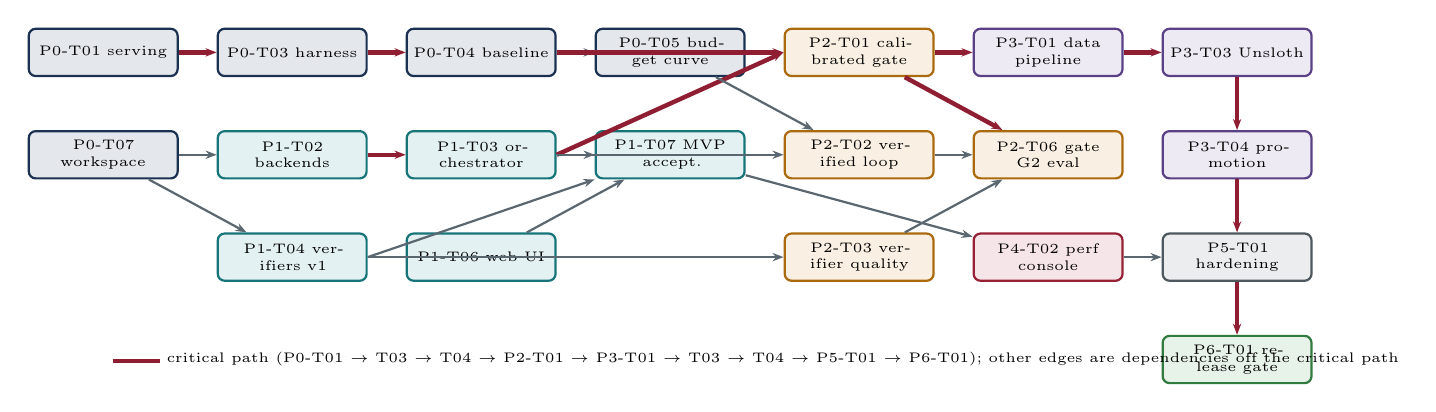
\begin{tikzpicture}[x=1cm,y=1cm]
\tikzset{tk/.style={sblk=#1,text width=1.75cm,minimum height=0.6cm},cp/.style={draw=crimson!80!black,line width=1.6pt}}
\node[tk=navy] (p0t1) at (0,0) {P0-T01 serving};
\node[tk=navy] (p0t3) at (2.4,0) {P0-T03 harness};
\node[tk=navy] (p0t4) at (4.8,0) {P0-T04 baseline};
\node[tk=navy] (p0t5) at (7.2,0) {P0-T05 budget curve};
\node[tk=navy] (p0t7) at (0,-1.3) {P0-T07 workspace};
\node[tk=teal] (p1t2) at (2.4,-1.3) {P1-T02 backends};
\node[tk=teal] (p1t3) at (4.8,-1.3) {P1-T03 orchestrator};
\node[tk=teal] (p1t7) at (7.2,-1.3) {P1-T07 MVP accept.};
\node[tk=teal] (p1t4) at (2.4,-2.6) {P1-T04 verifiers v1};
\node[tk=teal] (p1t6) at (4.8,-2.6) {P1-T06 web UI};
\node[tk=amber] (p2t1) at (9.6,0) {P2-T01 calibrated gate};
\node[tk=amber] (p2t2) at (9.6,-1.3) {P2-T02 verified loop};
\node[tk=amber] (p2t3) at (9.6,-2.6) {P2-T03 verifier quality};
\node[tk=amber] (p2t6) at (12.0,-1.3) {P2-T06 gate G2 eval};
\node[tk=violet] (p3t1) at (12.0,0) {P3-T01 data pipeline};
\node[tk=violet] (p3t3) at (14.4,0) {P3-T03 Unsloth};
\node[tk=violet] (p3t4) at (14.4,-1.3) {P3-T04 promotion};
\node[tk=crimson] (p4t2) at (12.0,-2.6) {P4-T02 perf console};
\node[tk=slate] (p5t1) at (14.4,-2.6) {P5-T01 hardening};
\node[tk=leaf] (p6t1) at (14.4,-3.9) {P6-T01 release gate};
\draw[arr,cp] (p0t1)--(p0t3); \draw[arr,cp] (p0t3)--(p0t4); \draw[arr] (p0t4)--(p0t5);
\draw[arr] (p0t7)--(p1t2); \draw[arr,cp] (p1t2)--(p1t3); \draw[arr] (p1t3)--(p1t7); \draw[arr] (p0t7)--(p1t4); \draw[arr] (p1t4.east)--(p1t7.south west);
\draw[arr] (p1t6)--(p1t7);
\draw[arr,cp] (p0t4)--(p2t1); \draw[arr,cp] (p1t3.east)--(p2t1.west);
\draw[arr] (p1t3.east)--(p2t2.west); \draw[arr] (p0t5)--(p2t2); \draw[arr] (p1t4)--(p2t3);
\draw[arr,cp] (p2t1)--(p2t6); \draw[arr] (p2t2)--(p2t6); \draw[arr] (p2t3)--(p2t6);
\draw[arr,cp] (p2t1)--(p3t1); \draw[arr,cp] (p3t1)--(p3t3); \draw[arr,cp] (p3t3)--(p3t4);
\draw[arr] (p1t7)--(p4t2); \draw[arr] (p4t2)--(p5t1); \draw[arr,cp] (p3t4)--(p5t1); \draw[arr,cp] (p5t1)--(p6t1);
\node[font=\tiny,anchor=west] at (0,-3.9) {\textcolor{crimson!80!black}{\rule{0.6cm}{1.6pt}} critical path (P0-T01 $\to$ T03 $\to$ T04 $\to$ P2-T01 $\to$ P3-T01 $\to$ T03 $\to$ T04 $\to$ P5-T01 $\to$ P6-T01); other edges are dependencies off the critical path};
\end{tikzpicture}
}\caption{Dependency graph of the main tasks with the critical path highlighted.}\label{fig:dep}\end{figure}
The critical path is P0-T01 $\to$ P0-T03 $\to$ P0-T04 $\to$ P2-T01 $\to$ P3-T01 $\to$ P3-T03 $\to$ P3-T04 $\to$ P5-T01 $\to$ P6-T01: the measurement baseline gates the calibrated gate, which gates the quality of the traces that feed training, which gates promotion, hardening and release. Work off the critical path (UI, bench console, dashboard, GPU profile) can absorb slack. Phase~1 overlaps Phase~0's baseline run because the baseline is machine-bound, not people-bound.

\section{Prioritised Backlog}
The full backlog (\NTasks\ tasks with MoSCoW priority, estimates, dependencies and requirement IDs) is exported to \texttt{backlog.csv} and \texttt{roadmap.md}. \textbf{Must} items are the critical path and the MVP; \textbf{Should} items are the judge hard gate, synthetic data, dashboard, drift monitor, replay mixing; \textbf{Could} items are budget mode, concurrency target, GPU scale-out, Profile~C and retrieval memory; \textbf{Won't} (this release): multimodal input, autonomous tool use beyond verifiers, diffusion decoding.

\section{Research-to-Engineering Plan}
\begin{table}[h]\centering\small\caption{Hypotheses from the formal model and their validation}
\begin{tabular}{@{}p{0.7cm}p{5.2cm}p{5.0cm}p{1.0cm}p{2.2cm}@{}}\toprule ID & Hypothesis (from result) & Experiment & Phase & Engineering effect if false\\\midrule
H1 & Calibrated gate reaches routing accuracy $\ge0.70$ at $g\le0.30$ (Thm.\,2, Prop.\,1) & labelled held-out set; oracle decisions; ECE and routing accuracy & 2 & richer features or budget mode; raise $\lambda$\\
H2 & Cascade costs $\le60\%$ of slow-only at matched accuracy (Prop.\,10) & paired runs over $\lambda$ grid; cost--accuracy curve & 2 & report honest frontier; adjust default $\lambda$\\
H3 & Per-task acceptance rates fit a Beta per domain (Prop.\,3) & goodness-of-fit on Phase-0 draws; compare predicted vs observed coverage & 2 & set $N$, $R$ from empirical coverage curve instead\\
H4 & Slow-path accuracy is concave in budget $b$ (Prop.\,9) & accuracy at $b\in\{128,256,512,1024,2048\}$ per domain & 0 & pick $b$ by grid search, not first-order condition\\
H5 & Draft-blind slow path adopts a wrong draft $<5\%$ (Prop.\,4) & $\ge200$ trials with seeded wrong drafts, both modes & 2 & keep draft-blind; investigate collision term\\
H6 & One distillation cycle gives LCB gain $>0$ without regression (Prop.\,7) & held-out verifier never used for collection; paired gate & 3 & more data, synthetic data, or no promotion\\
H7 & Qwen3.5 hybrid decodes at $\ge70\%$ of dense Qwen3 speed on the target CPU (Prop.\,8) & llama-bench, 4 threads, pp512/tg128 & 0 & stay on Profile~A\\
\bottomrule\end{tabular}\end{table}
Additional checks scheduled: the self-refinement fixed point of Theorem~4 (measure $u$, $d$ on a sample to confirm that unverified refinement is not monotone), the plurality floor of Theorem~6 (fraction of tasks with a wrong modal answer), and the audit-based self-model of Proposition~5 (compare audited against naive estimates).

\section{Where the Programme Stands and the Road Ahead}
\label{sec:ahead}
\textbf{Status on 18 October 2026.} Phases~0--6 are implemented on the CPU reference machine (GPU training and GPU scale-out deferred). Gate G5 passes. G1 passed earlier in the day but failed its latest run on NFR-004: the deliberate path took 354\,s against 240\,s while the host was shared. G4 fails on NFR-007 (concurrency on a shared four-core host, with the documented fallback). G0, G2, G3 and G6 are pending on release-scale sample sizes, the first GPU training cycle and the scholar review. Profile~C was evaluated and not adopted (more accurate, 3.7$\times$ slower). Latency attribution shows that System~1 decode speed dominates the fast path.

\begin{table}[h]\centering\small\caption{The road ahead (estimates; each phase keeps the gate discipline of Phases 0--7)}
\begin{tabular}{@{}p{2.6cm}p{6.3cm}p{6.2cm}@{}}\toprule Phase & Scope & Exit criteria\\\midrule
8 Evidence at scale & An idle or faster CPU host, or nightly slices: the 4\,600-task baseline, 700 paired items for G2, 2\,900 labelled drafts, 6\,200 pairs for G6; promote the calibrated gate and budget mode & G0, G2 and G6 closed with stored runs; ECE $\le0.05$; routing accuracy $\ge0.70$\\
9 Tazkiya cycle & 5\,000 verified traces (live and synthetic); the first Unsloth LoRA on a rented GPU; promotion under TR-007; rollback drill; re-fit the EAGLE-3 head to the distilled System~1 & G3 closed; LCB gain $>0$ without regression\\
10 Engine & EAGLE-3 or MTP speculation for both models; repacked 4-bit formats; adaptive early exit from System~2 reasoning; a router learned from the policy map and Both-trial preferences & decode speed-up $\ge1.2\times$ with identical greedy output; no accuracy loss on regression\_500\\
11 Product and review & Scholar review of the analogy text (SR-005); GPU profile for interactive deliberation; multilingual interface (Indonesian, Arabic); retrieval-grounded checks for open-domain answers & SR-005 signed off; slow-path p95 $\le20$\,s on the GPU profile\\
\bottomrule\end{tabular}\end{table}

\section{Success Metrics}
\begin{itemize}
\item \textbf{Phase 0:} baseline tables delivered; verifier $\hat\varphi\le0.01$; CI green.
\item \textbf{Phase 1:} MVP acceptance 9/9; NFR-002--NFR-005 met on the reference machine.
\item \textbf{Phase 2:} ECE $\le0.05$; routing accuracy $\ge0.70$; 3-point non-inferiority; cost ratio $\le0.60$; coupling $\le5\%$.
\item \textbf{Phase 3:} one gated training cycle completed; rollback $<1$ minute; zero privacy leaks on the seeded test.
\item \textbf{Phase 4:} full metric suite with tests; load reports at three concurrency levels; drift alarm sensitivity and specificity as specified.
\item \textbf{Phase 5:} no open high-severity findings; clean-host deployment; decisions on GPU and Profile~C recorded.
\item \textbf{Phase 6:} 1-point non-inferiority; documentation and publication delivered.
\item \textbf{Phase 7:} stage timings on every reply; interleaved A/B records for every serving change; early-escalation agreement $\ge95\%$; speculative heads adopted only with a measured speed-up.
\item \textbf{Phase 8:} a stored ROC study decides the gate's confidence signal; the window rule's early decisions equal full-draft decisions by construction (unit test of the running-minimum property); the posterior exit rule is default only after a paired Lab run; quantum-consciousness ideas are recorded with the test they failed.
\item \textbf{Programme:} a CPU-only dual-process assistant whose answers carry honest assurance levels, whose gate is derived and calibrated, whose precision on verifiable tasks is bounded by measured verifier rates, and whose fast path improves through a gated distillation loop, with every claim traceable to a stored evaluation run.
\end{itemize}
\end{document}
